% =============================================================================
%  BARISTA — BARrier Inference of Sequential, Tunnelling & Activated transport
%  Feature presentation (LaTeX Beamer, 16:9).  Build:  ./build.sh   (or latexmk -pdf)
%  Colour code used in every equation:
%     bias V (green) · temperature T (purple) · thickness d (orange) · current I, J (blue)
%     trap / state densities N (red) · energies Φ, E (brown) · spin quantities (magenta)
%     operators: d/dln, exp, sinh, ∫, softmax ... (teal)
% =============================================================================
\documentclass[aspectratio=169,10pt]{beamer}
\usetheme[progressbar=frametitle,numbering=fraction,block=fill]{metropolis}
\usepackage[T1]{fontenc}
\usepackage[utf8]{inputenc}
\usepackage{amsmath,amssymb,bm}
\usepackage{booktabs,tabularx,array,multirow}
\usepackage{graphicx}
\usepackage{tikz}
\usetikzlibrary{arrows.meta,positioning,shapes.geometric,calc,fit,backgrounds}
\usepackage{xcolor}
\usepackage{listings}
\graphicspath{{figs/}}

% ---------------- palette -----------------------------------------------------
\definecolor{navy}{HTML}{1F3A5F}
\definecolor{acc}{HTML}{2A78D6}
\definecolor{soft}{HTML}{F4F3EF}
\definecolor{ink2}{HTML}{52514E}
\definecolor{okgreen}{HTML}{1B8A3A}
\definecolor{bad}{HTML}{C0392B}
% physical quantities
\definecolor{cV}{HTML}{1B8A3A}   % bias
\definecolor{cT}{HTML}{6A3DA8}   % temperature
\definecolor{cd}{HTML}{D9661F}   % thickness
\definecolor{cI}{HTML}{1F5FBF}   % current
\definecolor{cN}{HTML}{C0392B}   % densities (traps, states)
\definecolor{cE}{HTML}{8A5A14}   % energies
\definecolor{cS}{HTML}{B0307A}   % spin
\definecolor{cO}{HTML}{0F7C7C}   % operators

\newcommand{\qV}{{\color{cV}V}}
\newcommand{\qF}{{\color{cV}F}}
\newcommand{\qT}{{\color{cT}T}}
\newcommand{\qd}{{\color{cd}d}}
\newcommand{\qI}{{\color{cI}I}}
\newcommand{\qJ}{{\color{cI}J}}
\newcommand{\qG}{{\color{cI}G}}
\newcommand{\qN}[1][t]{{\color{cN}N_{#1}}}
\newcommand{\qE}[1]{{\color{cE}#1}}
\newcommand{\qS}[1]{{\color{cS}#1}}
\newcommand{\op}[1]{{\color{cO}#1}}

\setbeamercolor{frametitle}{bg=navy,fg=white}
\setbeamercolor{progress bar}{fg=acc,bg=soft}
\setbeamercolor{title separator}{fg=acc}
\setbeamercolor{alerted text}{fg=acc}
\setbeamercolor{block title}{bg=navy!12,fg=navy}
\setbeamercolor{block body}{bg=soft}
\setbeamercolor{block title example}{bg=okgreen!15,fg=okgreen!70!black}
\setbeamercolor{block body example}{bg=okgreen!5}
\setbeamercolor{block title alerted}{bg=bad!15,fg=bad}
\setbeamercolor{block body alerted}{bg=bad!4}
\setbeamerfont{frametitle}{size=\large,series=\bfseries}
\setbeamertemplate{itemize item}{\color{acc}\small$\blacktriangleright$}
\setbeamertemplate{itemize subitem}{\color{ink2}\tiny$\bullet$}

\lstset{basicstyle=\ttfamily\scriptsize,keywordstyle=\color{acc}\bfseries,commentstyle=\color{ink2}\itshape,
        stringstyle=\color{cd},backgroundcolor=\color{soft},frame=single,rulecolor=\color{soft},
        breaklines=true,columns=fullflexible,showstringspaces=false,xleftmargin=4pt,xrightmargin=4pt}

\newcommand{\badge}[2][acc]{\tikz[baseline=(t.base)]\node[fill=#1!15,text=#1!80!black,rounded corners=2pt,
  inner sep=2pt,font=\scriptsize\bfseries](t){#2};}
\newcommand{\src}[1]{\par\vfill{\tiny\color{ink2}#1}}

\title{BARISTA}
\subtitle{BARrier Inference of Sequential, Tunnelling \& Activated transport}
\author{Gokaran Shukla}
\institute{King Abdullah University of Science and Technology (KAUST), Thuwal\\
\href{https://github.com/Gokaran-Shukla/barista}{\texttt{github.com/Gokaran-Shukla/barista}} \quad version 0.3.0}
\date{Transport-mechanism identification across thin barriers from $\qI(\qV,\qT,\qd)$ data\\[2pt] November 2026}

\begin{document}

% =============================================================================
\begin{frame}
  \titlepage
\end{frame}

% =============================================================================
\begin{frame}{The problem}
\begin{columns}[T]
\column{0.53\textwidth}
\begin{itemize}
  \item A single $\qI(\qV)$ curve is usually compatible with \alert{several mechanisms}: tunnelling, hopping,
        emission and space-charge currents can all look similar over a decade of bias.
  \item Published assignments often rest on one linearised plot (``$\ln \qI$ vs $\sqrt{\qV}$ is straight'').
  \item The distinguishing information is in the \alert{joint} dependence on bias, temperature and thickness.
  \item Extracted parameters ($\qE{\Phi}$, $\qN$, $\varepsilon_r$, $\xi$, \dots) are only meaningful if the mechanism is right.
\end{itemize}
\column{0.44\textwidth}
\begin{block}{What BARISTA does}
\small
\begin{enumerate}
  \item Reads any $\qI$--$\qV$ file (or a published paper).
  \item Measures model-free fingerprints.
  \item Fits 13 physical mechanisms globally.
  \item Ranks them, states a verdict and how certain it is.
  \item Extracts parameters with 95\,\% intervals, including the \alert{trap density}.
  \item Exports manuscript-ready figures and tables.
\end{enumerate}
\end{block}
\end{columns}
\src{Protocol and formula sheets follow G. Shukla, ``Charge transport mechanisms across thin barriers: theory and experimental fingerprints'' (2026).}
\end{frame}

% =============================================================================
\begin{frame}{Pipeline}
\centering
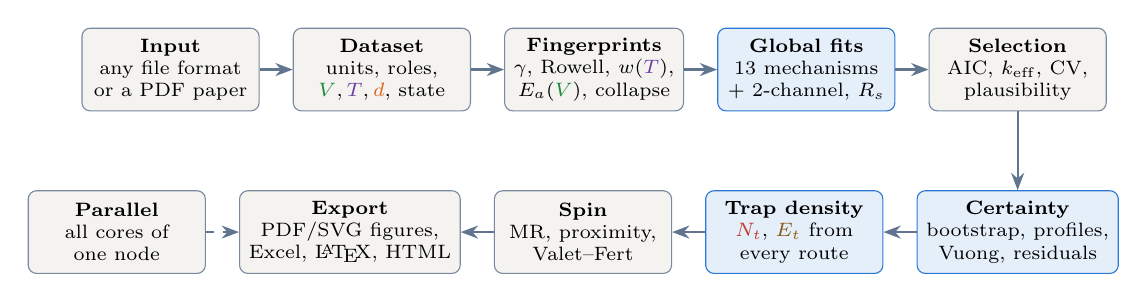
\begin{tikzpicture}[
  box/.style={draw=navy!60,fill=soft,rounded corners=3pt,minimum width=2.25cm,minimum height=1.05cm,
              align=center,font=\scriptsize},
  hl/.style={box,fill=acc!12,draw=acc},
  arr/.style={-{Stealth[length=2.2mm]},thick,color=navy!70},
  node distance=0.42cm and 0.42cm]
\node[box] (in) {\textbf{Input}\\any file format\\or a PDF paper};
\node[box,right=of in] (ds) {\textbf{Dataset}\\units, roles,\\$\qV,\qT,\qd$, state};
\node[box,right=of ds] (fp) {\textbf{Fingerprints}\\$\gamma$, Rowell, $w(\qT)$,\\$E_a(\qV)$, collapse};
\node[hl,right=of fp] (fit) {\textbf{Global fits}\\13 mechanisms\\+ 2-channel, $R_s$};
\node[box,right=of fit] (sel) {\textbf{Selection}\\AIC, $k_\mathrm{eff}$, CV,\\plausibility};
\node[hl,below=1.0cm of sel] (cert) {\textbf{Certainty}\\bootstrap, profiles,\\Vuong, residuals};
\node[hl,left=of cert] (trap) {\textbf{Trap density}\\$\qN$, $\qE{E_t}$ from\\every route};
\node[box,left=of trap] (spin) {\textbf{Spin}\\MR, proximity,\\Valet--Fert};
\node[box,left=of spin] (out) {\textbf{Export}\\PDF/SVG figures,\\Excel, \LaTeX, HTML};
\node[box,left=of out] (hpc) {\textbf{Parallel}\\all cores of\\one node};
\draw[arr] (in)--(ds); \draw[arr] (ds)--(fp); \draw[arr] (fp)--(fit); \draw[arr] (fit)--(sel);
\draw[arr] (sel)--(cert); \draw[arr] (cert)--(trap); \draw[arr] (trap)--(spin); \draw[arr] (spin)--(out);
\draw[arr,dashed] (hpc)--(out);
\end{tikzpicture}
\vspace{0.4cm}

\small Three interfaces on the same engine: command line \texttt{barista}, Streamlit GUI, Python API.
\end{frame}

% =============================================================================
\section{Input data}

\begin{frame}{Reads every kind of input file}
\begin{columns}[T]
\column{0.5\textwidth}
\textbf{Formats}
\begin{itemize}\small
  \item Text: CSV, TSV, DAT, TXT --- any delimiter, decimal commas, instrument headers (Keithley, Keysight, \dots)
  \item Excel / ODS (every sheet), JSON, HDF5, MATLAB \texttt{.mat}, NumPy, Parquet, Feather, Pickle
  \item ZIP / TAR archives and whole folders
  \item PDF papers and figure images (see \emph{Paper reader})
\end{itemize}
\textbf{Layouts}
\begin{itemize}\small
  \item long (one row per point), wide (one column per $\qT$ or $\qd$), paired $\qV$/$\qI$ columns
\end{itemize}
\column{0.47\textwidth}
\textbf{Automatic role detection} from names and units
\begin{itemize}\small
  \item $\qV$ [V, mV], $\qI$ [A, mA, nA], $\qJ$ [A\,cm$^{-2}$]
  \item $\qT$ [K, \textdegree C], $\qd$ [nm, \AA, layers $N$]
  \item area, magnetic state (P/AP), angle, MR
  \item values taken from file names / headers (e.g. \texttt{d=5nm\_T300K.csv})
\end{itemize}
\begin{exampleblock}{Coverage report}
\small The dataset reports how many temperatures, thicknesses and curves were found --- this decides which
tests are possible.
\end{exampleblock}
\end{columns}
\end{frame}

\begin{frame}{Optional device information}
\small
All inputs are optional. By default they are starting values and consistency checks; with \texttt{--fix} they become hard constraints.
\vspace{4pt}

\begin{columns}[T]
\column{0.49\textwidth}
\footnotesize
\begin{tabularx}{\linewidth}{>{\ttfamily}l X}
\toprule
\normalfont\bfseries option & \bfseries meaning\\
\midrule
--area            & junction area (\textmu m$^2$)\\
--thickness       & $\qd$ if not in the file\\
--temperature     & $\qT$ if not in the file\\
--eps-r, --n-opt  & static / optical permittivity\\
--barrier, --mass & $\qE{\Phi}$, $m^*/m_e$\\
--band-gap        & $\qE{E_g}$ (band-to-band)\\
--layer-spacing   & interlayer spacing $a$\\
\bottomrule
\end{tabularx}
\column{0.49\textwidth}
\footnotesize
\begin{tabularx}{\linewidth}{>{\ttfamily}l X}
\toprule
\normalfont\bfseries option & \bfseries meaning\\
\midrule
--trap-density    & $\qN$ (cm$^{-3}$), checked vs prediction\\
--trap-depth      & $\qE{E_c-E_t}$ or $\qE{\Phi_t}$\\
--mobility        & $\mu$ (cm$^2$/Vs)\\
--attempt-freq    & $\nu_0$ (trap-assisted tunnelling)\\
--material        & prior class (oxide, vdW, organic, \dots)\\
--layers, --system & $N$ layers; system preset\\
--exchange, --ordering-T & spin starting values\\
\bottomrule
\end{tabularx}
\end{columns}
\vspace{6pt}

System presets: \texttt{graphene/crsb/graphene} ($a=0.2735$\,nm), \texttt{graphite/cri3/graphite},
\texttt{graphite/crsbr/graphite}, \texttt{cofeb/mgo/cofeb}.
\end{frame}

% =============================================================================
\section{Mechanisms and fingerprints}

\begin{frame}{Thirteen mechanisms, one consistent framework}
\scriptsize\renewcommand{\arraystretch}{0.9}
\begin{tabularx}{\textwidth}{l X l}
\toprule
\textbf{Mechanism} & \textbf{Model (global in $\qV,\qT,\qd$)} & \textbf{Key parameters}\\
\midrule
Coherent tunnelling & Tsu--Esaki + WKB; covers direct, Fowler--Nordheim, thermionic-field, thermionic & $\qE{\Phi}$, $m^*$\\
Trap-assisted tunnelling & two-step elastic, $\qJ\propto \qN\op{\int} T_1T_2/(T_1+T_2)\,\mathrm{d}x$ & $\qE{\Phi_t}$, $\qN$\\
Glazman--Matveev & resonant chains, $\qG_N\propto \qT^{\,N-2/(N+1)}$ & $\xi$, $c_N$\\
Band-to-band & Kane, $\qJ\propto \qF^2\op{\exp}(-B\qE{E_g}^{3/2}/\qF)$ & $\qE{E_g}$, $m^*$\\
Schottky & $\qJ\propto \qT^2\op{\exp}[-(\qE{\Phi_B}-\beta_S\sqrt{\qF})/k\qT]$ & $\qE{\Phi_B}$, $\varepsilon_r$\\
Poole--Frenkel & $\qJ\propto \qF\op{\exp}[-(\qE{\Phi_t}-\beta_{PF}\sqrt{\qF})/k\qT]$ & $\qE{\Phi_t}$, $\varepsilon_r$\\
NN / ionic hopping & $\qJ\propto \op{\exp}(-\qE{E_a}/k\qT)\op{\sinh}(e\qF r/2k\qT)$ & $\qE{E_a}$, $r$\\
Variable-range hopping & $\sigma\propto\op{\exp}[-(\qT_0/\qT)^p]$, field-assisted & $\qT_0$, $p$, $\xi$\\
Polaron (Marcus) & $\op{\exp}[-(\lambda-ea\qF)^2/4\lambda k\qT]$ & $\lambda$, $a$\\
Gaussian disorder & B\"assler GDM mobility & $\sigma$, $\Sigma$\\
SCLC, discrete trap & \alert{exact drift--Poisson}, one level, ohmic $\to\theta\qV^2/\qd^3\to$ TFL $\to$ Mott--Gurney & $\qN$, $\qE{E_c-E_t}$, $\mu$\\
SCLC, exponential & Mark--Helfrich, $\qJ\propto \qV^{\,l+1}/\qd^{\,2l+1}$ & $\qN$, $k\qT_c$\\
Ohmic / metallic & $\qG(\qT)=\qG_0[1-\alpha(\qT-\qT_0)]$ & $\alpha$\\
\bottomrule
\end{tabularx}
\vspace{2pt}

Each model carries plausibility checks (e.g.\ $\varepsilon_r$ vs $n^2$, physical mass, trap depth vs barrier).
\end{frame}

\begin{frame}{Model-free fingerprints, measured before any fit}
\begin{columns}[T]
\column{0.42\textwidth}
\small
\begin{itemize}
  \item Logarithmic derivative
  \[\gamma=\op{\frac{\mathrm{d}\ln}{\mathrm{d}\ln}}\frac{\qI}{\qV}\ \text{(ohmic 1, SCLC 2, TFL peak)}\]
  \item Rowell ratio $\qG(\qT_\mathrm{hi})/\qG(\qT_\mathrm{lo})$
  \item Zabrodskii $w=\op{\frac{\mathrm{d}\ln}{\mathrm{d}\ln}}\frac{\sigma}{\qT}=p(\qT_0/\qT)^p$
  \item Arrhenius $\qE{E_a}(\qV)$ vs $\sqrt{\qV}$; slope gives $\varepsilon_r$
  \item Thickness collapse: $\qJ$ vs $\qV/\qd$ (field) or $\qJ/\qd$ vs $\qV/\qd^2$ (SCLC)
  \item FN transition voltage, hysteresis, NDR, zero-bias gap
\end{itemize}
\column{0.56\textwidth}
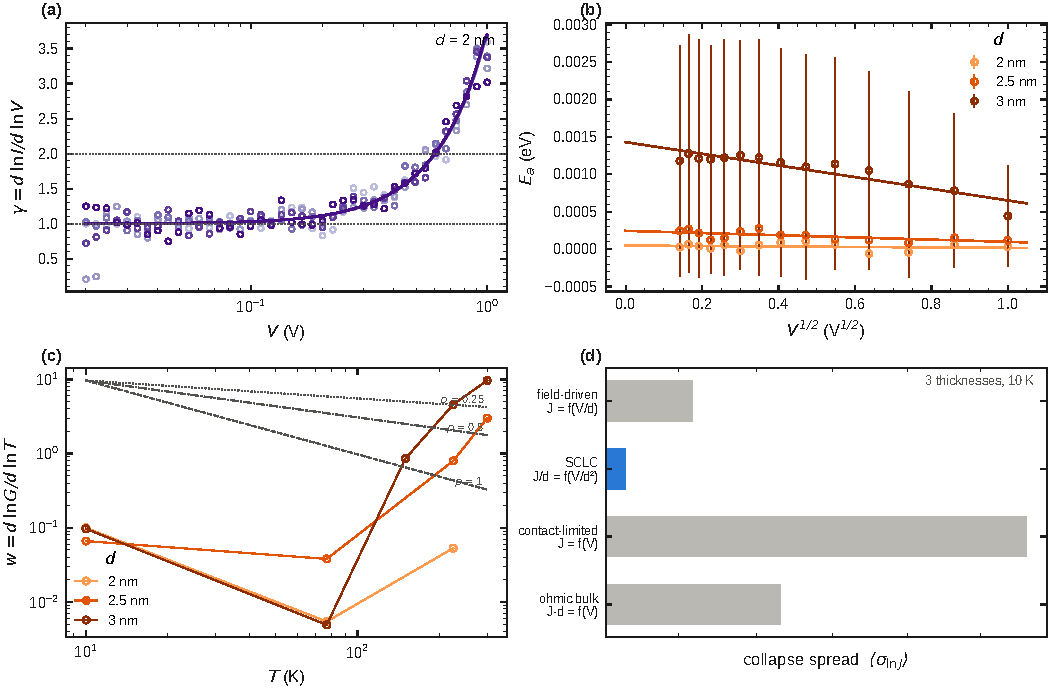
\includegraphics[width=\linewidth]{mixed_fig3.pdf}
\end{columns}
\end{frame}

% =============================================================================
\section{Fitting and decision}

\begin{frame}{Global fitting and model selection}
\begin{columns}[T]
\column{0.5\textwidth}
\small
\textbf{Fitting}
\begin{itemize}
  \item One parameter set for \emph{all} curves; residuals in $\ln\qI$
  \item Prefactor profiled analytically; multi-start trust-region least squares
  \item Effective parameter count $k_\mathrm{eff}$ from the Jacobian rank
  \item Cross-validation: leave one $\qT$ (or $\qd$) out and predict it
  \item Two-channel $A\parallel B$ models and a series-resistance model
\end{itemize}
\column{0.47\textwidth}
\small
\textbf{Score and support}
\[
S_m=-\tfrac12\op{\min}(\Delta\mathrm{AIC}_m,80)+\mathcal{E}_m+\mathcal{P}_m+\mathcal{C}_m
\]
\[
p_m=\op{\mathrm{softmax}}(S_m)
\]
\scriptsize $\mathcal{E}$: fingerprint evidence; $\mathcal{P}$: plausibility; $\mathcal{C}$: cross-validation.

\vspace{4pt}
\small\textbf{Verdicts}\\[2pt]
\badge[okgreen]{IDENTIFIED} \badge{MOST LIKELY} \badge[cd]{LEADING CANDIDATE} \badge[bad]{EXCLUDED}\\[3pt]
\scriptsize Bias-only data are capped at ``leading candidate --- not identifiable from bias alone'';
IDENTIFIED requires a good fit.
\end{columns}
\end{frame}

\begin{frame}{Example: two channels in Al/AlO$_x$ junctions}
\centering
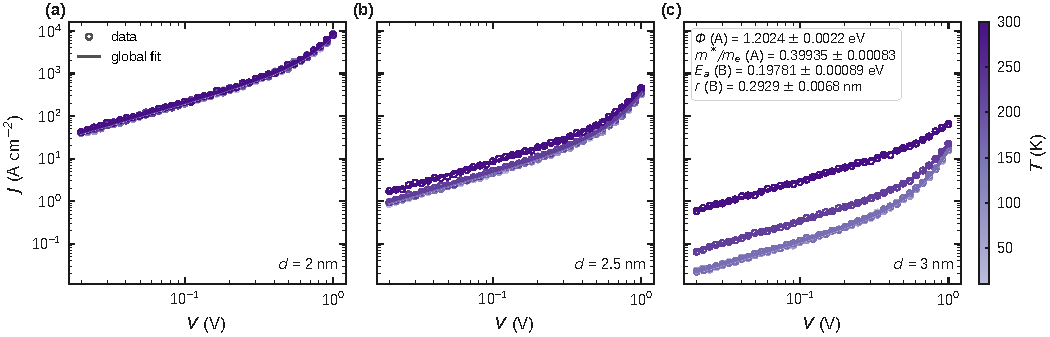
\includegraphics[height=0.30\textheight]{mixed_fig1.pdf}\\[2pt]
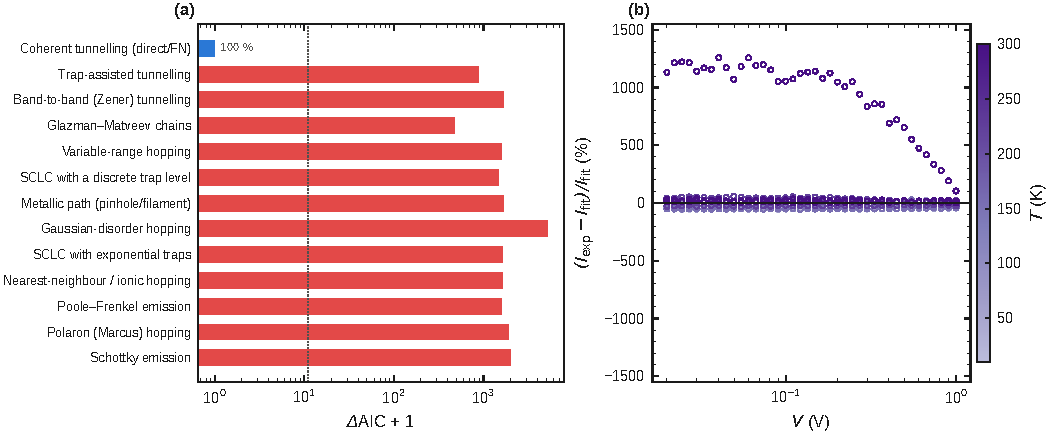
\includegraphics[height=0.38\textheight]{mixed_fig4.pdf}
\src{Example data shipped in \texttt{examples/mixed\_channels}. Top: global fit of the assigned model; bottom: $\Delta$AIC of every candidate and residuals.}
\end{frame}

\begin{frame}{Regimes and falsifiable predictions}
\begin{columns}[c]
\column{0.62\textwidth}
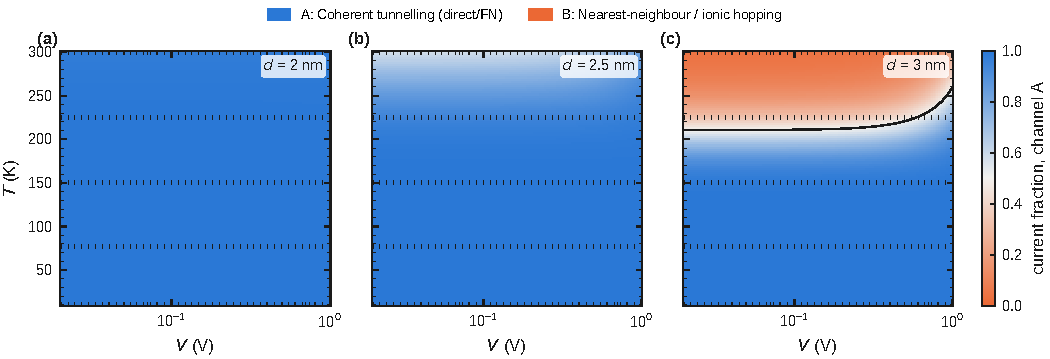
\includegraphics[width=\linewidth]{mixed_fig5.pdf}
\column{0.36\textwidth}
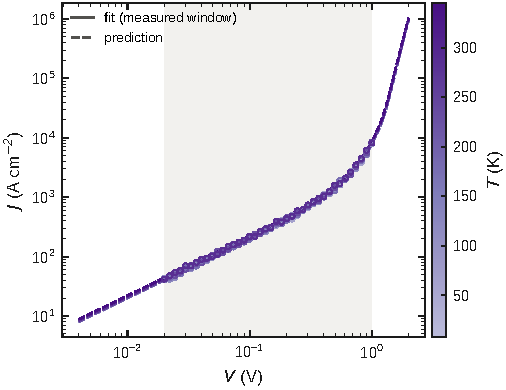
\includegraphics[width=\linewidth]{mixed_fig6.pdf}
\end{columns}
\vspace{4pt}
\small
\begin{itemize}
  \item Sub-regime map: which limit (direct / FN / thermionic, or which channel) dominates at each $(\qV,\qT)$.
  \item Extrapolation outside the measured window --- a prediction you can test with one more measurement.
  \item The report also proposes the \alert{next measurements} that would separate the remaining candidates.
\end{itemize}
\end{frame}

% =============================================================================
\section{How certain is the assignment?}

\begin{frame}{Statistical certainty analysis}
\begin{columns}[T]
\column{0.48\textwidth}
\small
\begin{itemize}
  \item \textbf{Stratified bootstrap} (resampling within each curve): probability that each mechanism is selected, with Wilson 95\,\% intervals
  \item \textbf{Akaike weights} and \textbf{BIC posteriors}
  \item \textbf{Profile likelihood}: $\Delta\chi^2 = 1$ and $3.84$
  \item Asymptotic intervals with Student-$t$
  \item \textbf{Fit-window stability} of each parameter
  \item Residual tests: Shapiro--Wilk, Durbin--Watson, runs
  \item \textbf{Vuong} (non-nested) and likelihood-ratio tests
\end{itemize}
\vspace{2pt}
Overall grade: \badge[bad]{LOW} \badge[cd]{MODERATE} \badge{HIGH} \badge[okgreen]{VERY HIGH}
\column{0.5\textwidth}
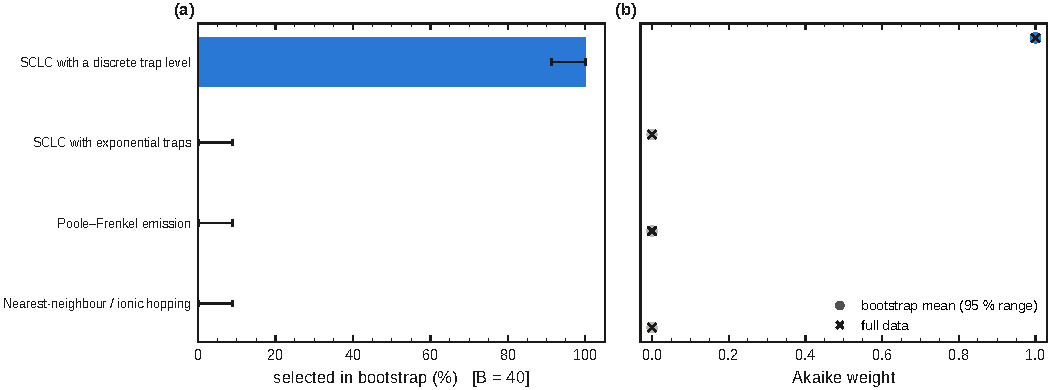
\includegraphics[width=\linewidth]{sclc_fig8_model_certainty.pdf}
\end{columns}
\end{frame}

\begin{frame}{Parameter intervals that can be trusted}
\begin{columns}[c]
\column{0.38\textwidth}
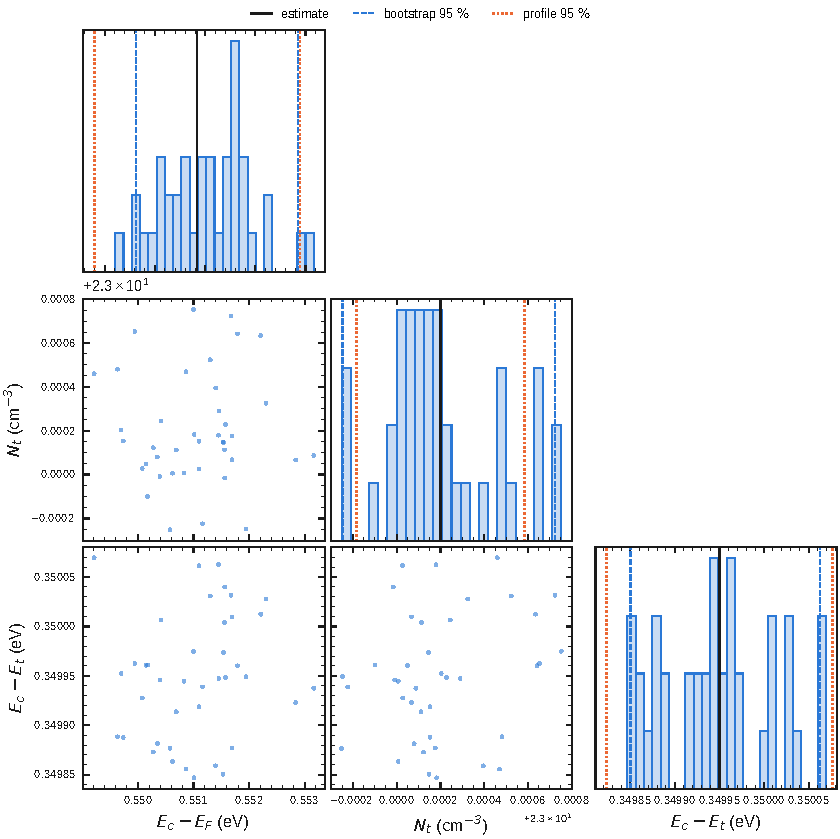
\includegraphics[width=\linewidth]{sclc_fig9_parameter_uncertainty.pdf}
\column{0.58\textwidth}
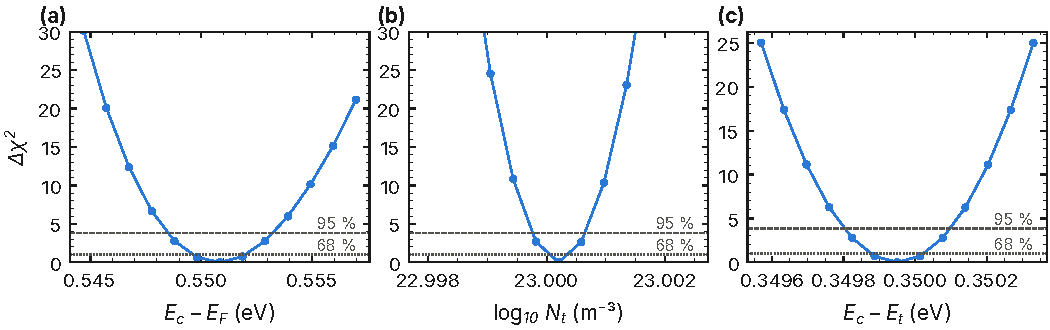
\includegraphics[width=0.92\linewidth]{sclc_fig10_profile_likelihood.pdf}\\[4pt]
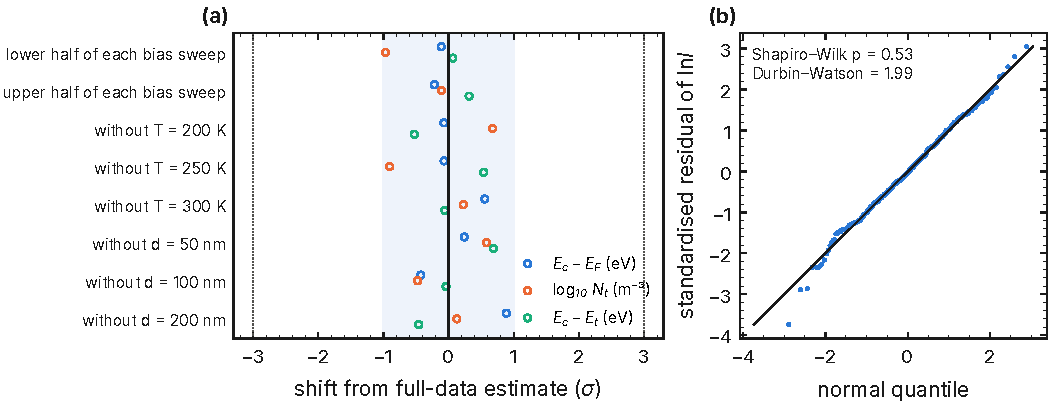
\includegraphics[width=0.92\linewidth]{sclc_fig11_stability_residuals.pdf}
\end{columns}
\src{SCLC device with planted $\qN=10^{17}$\,cm$^{-3}$, $\qE{E_c-E_t}=0.35$\,eV: bootstrap distributions and correlations, profile likelihoods, window stability and residual normality.}
\end{frame}

% =============================================================================
\section{Trap density from the I--V data}

\begin{frame}{Trap density and trap energy --- whatever the mechanism}
\scriptsize
\begin{tabularx}{\textwidth}{l X l}
\toprule
\textbf{Mechanism} & \textbf{Route to $\qN$} & \textbf{Energy}\\
\midrule
SCLC, single level & exact drift--Poisson fit & $\qE{E_c-E_t}$\\
SCLC, any & model-free trap-filled limit $\qN=\dfrac{2\varepsilon\,\qV_\mathrm{TFL}}{e\,\qd^{\,2}}$ from the $\gamma$ peak; test $\qV_\mathrm{TFL}\propto\qd^{\,2}$ & ---\\[4pt]
SCLC, exponential tail & total $\qN$ (Mark--Helfrich) & $k\qT_c$\\
Trap-assisted tunnelling & $\qN=C/(e\nu_0)$, $\nu_0=10^{12}$--$10^{14}$\,s$^{-1}$ & $\qE{\Phi_t}$\\
NN / ionic / polaron hopping & site density $\qN\approx 3/(4\pi r^3)$ from the hop length & $\qE{E_a}$\\
Variable-range hopping & $g(\qE{E_F})=\dfrac{21.2}{k\qT_0\,\xi^3}$; states in the hopping band $g\,\Delta\qE{E_h}(\qT)$ & $\Delta\qE{E_h}$\\[4pt]
Poole--Frenkel & depth exact; $\qN<1/(2x_m)^3$; absolute $\qN$ with $\mu$ & $\qE{\Phi_t}$\\
Coherent, Schottky, metallic & \alert{no traps needed}; 95\,\% upper bound from a parallel TAT channel & ---\\
\bottomrule
\end{tabularx}
\vspace{4pt}

\small 95\,\% intervals from the bootstrap; support-weighted consensus; a supplied \texttt{--trap-density} is
checked; for papers, compared with the value the authors quote.
\end{frame}

\begin{frame}{Trap density: validation}
\centering
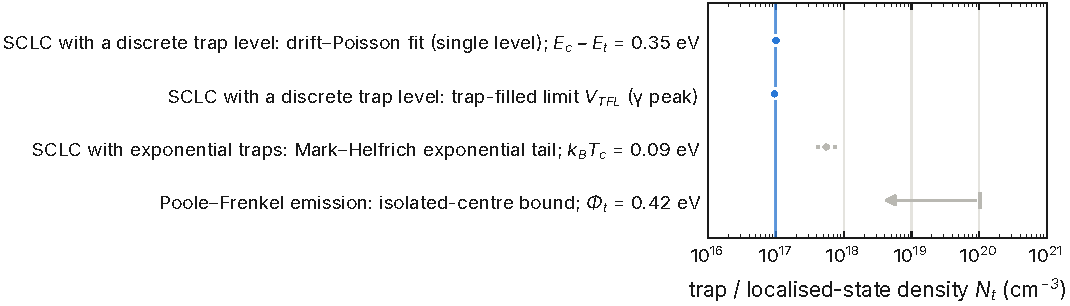
\includegraphics[width=0.86\linewidth]{sclc_fig15_trap_density.pdf}
\vspace{4pt}

\scriptsize
\begin{tabular}{lccc}
\toprule
Mechanism (synthetic, known truth) & true $\qN$ (cm$^{-3}$) & recovered & energy true $\to$ recovered\\
\midrule
SCLC, single level & $1.0\times10^{17}$ & $1.0\times10^{17}$ (fit) / $9.5\times10^{16}$ ($\gamma$ peak) & 0.35 $\to$ 0.350 eV\\
SCLC, exponential tail & $3.2\times10^{17}$ & $3.2\times10^{17}$ & 77.6 $\to$ 77.5 meV\\
Trap-assisted tunnelling & $6.2\times10^{11}$ & $6.2\times10^{11}$ & 1.0 $\to$ 1.0 eV\\
NN hopping & $7.1\times10^{19}$ & $7.1\times10^{19}$ & 0.12 $\to$ 0.12 eV\\
VRH, $g(E_F)$ (eV$^{-1}$cm$^{-3}$) & $2.5\times10^{20}$ & $2.5\times10^{20}$ & ---\\
\bottomrule
\end{tabular}
\end{frame}

% =============================================================================
\section{Spin-dependent transport}

\begin{frame}{Spin-dependent transport models}
\begin{columns}[T]
\column{0.52\textwidth}
\small
\begin{itemize}
  \item \textbf{Jullière}: $\mathrm{TMR}=\dfrac{2\qS{P_1P_2}}{1-\qS{P_1P_2}}$
  \item \textbf{Layered spin filter} ($N$ layers, spacing $a$):\\
        $1+\mathrm{MR}=\op{\cosh}(Na\qS{\Delta\kappa})$ \ (even $N$)\\
        $1+\mathrm{MR}=\op{\cosh}(Na\qS{\Delta\kappa})/\op{\cosh}(a\qS{\Delta\kappa})$ \ (odd $N$)
  \item \textbf{Spin-dependent hopping}: $\mathrm{MR}=\op{\exp}(\Delta\qE{E_a}/k\qT)-1$
  \item \textbf{Interface proximity polarisation}: spin-split Dirac-cone electrodes, exchange $\qS{\Delta}$, chemical potential $\mu$, broadening $\Gamma$, $\qS{\Delta}(\qT)$ vanishing at $\qT_N$
  \item \textbf{Valet--Fert / Fert--Jaffrès} exact CPP drift--diffusion: bulk $\beta$, interface $\gamma$, spin-diffusion length $\qS{l_{sf}}$
\end{itemize}
\column{0.45\textwidth}
\begin{block}{Graphene/CrSb/graphene}
\small
\begin{itemize}
  \item choose the number of CrSb layers $N$ (\texttt{--layers})
  \item supply or fit the trap density
  \item P/AP (or angle) columns trigger the spin analysis automatically
  \item MR vs $\qV$, $\qT$ and $N$ separate \emph{interface} from \emph{barrier} spin filtering
\end{itemize}
\end{block}
\end{columns}
\end{frame}

\begin{frame}{Interface polarisation from the exchange field}
\centering
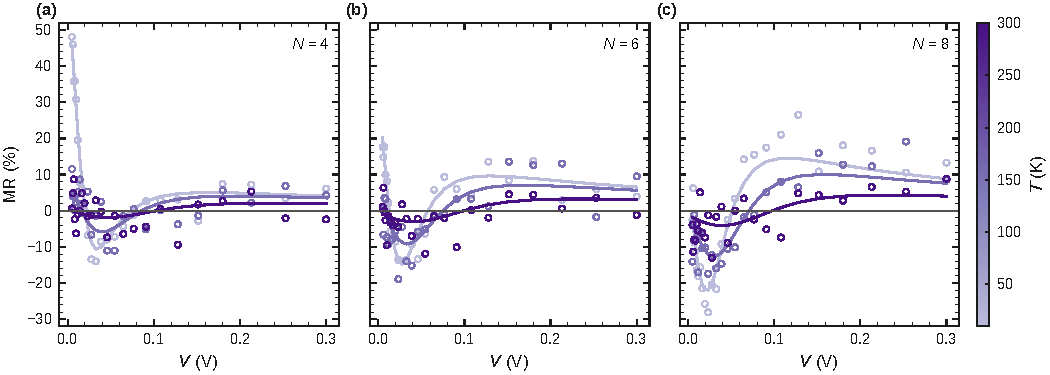
\includegraphics[height=0.37\textheight]{fig12_spin_MR_bias.pdf}\\[2pt]
\begin{columns}[c]
\column{0.48\textwidth}
\centering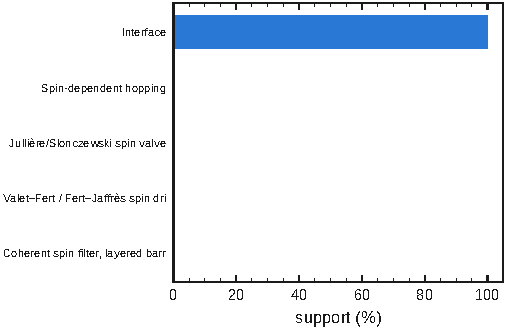
\includegraphics[height=0.36\textheight]{fig14_spin_models.pdf}
\column{0.5\textwidth}
\small
Hidden truth $\qS{\Delta}=20$\,meV, $\mu=15$\,meV:\\[2pt]
\textbf{recovered} $\qS{\Delta}=19.3\,[17.4, 20.7]$\,meV,\\
\phantom{\textbf{recovered} }$\mu=14.7\,[13.8, 16.0]$\,meV.\\[4pt]
MR changes sign with bias and is independent of $N$: the fingerprint of an \alert{interface} (proximity) term.
\end{columns}
\end{frame}

\begin{frame}{Layer-number scaling}
\centering
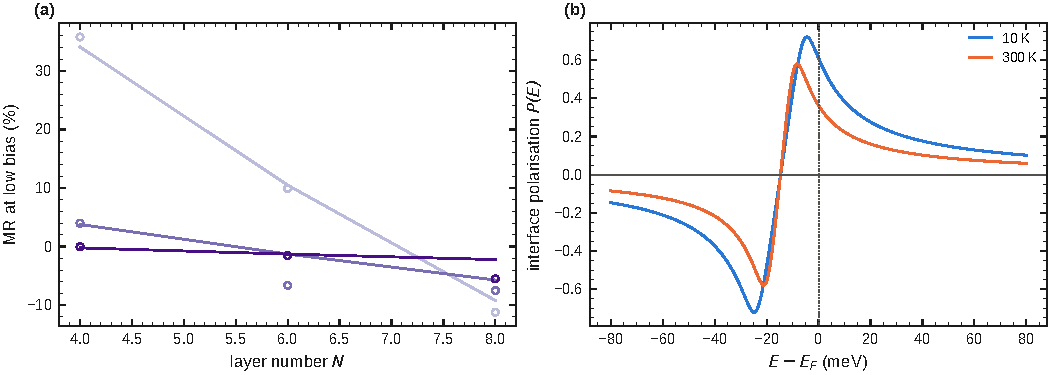
\includegraphics[height=0.47\textheight]{fig13_spin_scaling.pdf}
\vspace{4pt}

\footnotesize
\begin{tabular}{lll}
\toprule
Benchmark & Published & BARISTA (95\,\% CI)\\
\midrule
CrI$_3$ spin filter (Klein 2018) & $a\qS{\Delta\kappa}\approx0.64$--$0.78$ & $0.660\ [0.619, 0.713]$\\
CrSBr spin hopping (Lin 2024) & $\Delta\qE{E_a}=20$ meV & $19.99\ [19.97, 20.01]$ meV\\
F/I/N/I/F Fert--Jaffrès (synthetic) & $\gamma=0.6$, $\qS{l_{sf}}=300$ nm & $\gamma=0.75\ [0.54, 0.77]$, $\qS{l_{sf}}=365\ [284, 521]$ nm\\
\bottomrule
\end{tabular}
\end{frame}

% =============================================================================
\section{Reading published papers}

\begin{frame}[fragile]{Paper reader: from PDF to mechanism}
\begin{columns}[T]
\column{0.55\textwidth}
\small
\begin{enumerate}
  \item \textbf{Text}: title, DOI, abstract, captions; authors' claimed mechanism; reported parameters
        ($\qE{\Phi}$, $\qN$, $\varepsilon_r$, \dots)
  \item \textbf{Vector figures}: axis frames, tick labels (incl.\ $10^n$), calibration, every coloured series, legend
  \item \textbf{Raster figures}: frame detection, OCR of ticks and legends, colour clustering in Lab space
  \item \textbf{Analysis}: the full BARISTA pipeline on each digitised dataset
  \item \textbf{Verdict vs authors}: \badge[okgreen]{AGREES} \badge{SAME FAMILY} \badge[cd]{DATA CANNOT DECIDE} \badge[bad]{DISAGREES}
\end{enumerate}
\begin{lstlisting}[language=bash]
barista paper article.pdf -o paper_out --bootstrap 200
\end{lstlisting}
\column{0.42\textwidth}
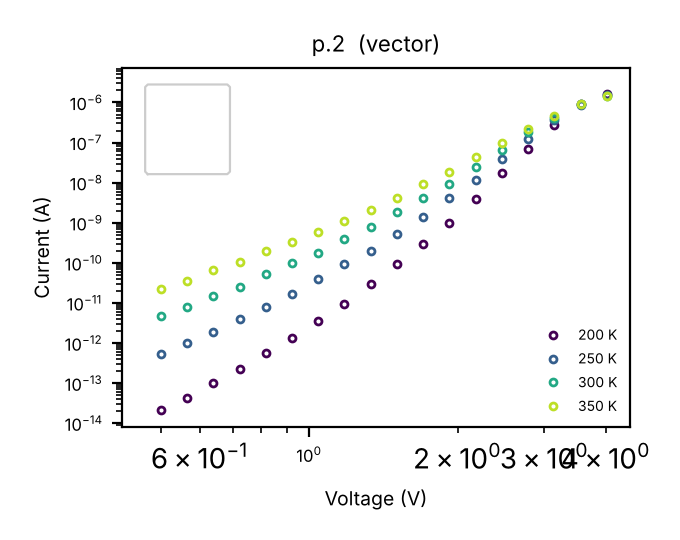
\includegraphics[width=\linewidth]{digitised_figures.png}
\end{columns}
\end{frame}

\begin{frame}{Digitiser accuracy and mock-paper test}
\begin{columns}[T]
\column{0.47\textwidth}
\small\textbf{Digitiser} (all series recovered)\\[3pt]
\scriptsize
\begin{tabular}{lcc}
\toprule
Axes & vector & raster 300 dpi\\
\midrule
log--log & $2\times10^{-5}$ & 0.6\,\%\\
linear--log & $1.4\times10^{-4}$ & 0.7\,\%\\
linear--linear & $1\times10^{-5}$ & 1.1\,\%\\
log--log (dense) & $1.2\times10^{-4}$ & 1.9\,\%\\
\bottomrule
\end{tabular}\\[2pt]
\scriptsize median relative error in $\qI$
\vspace{6pt}

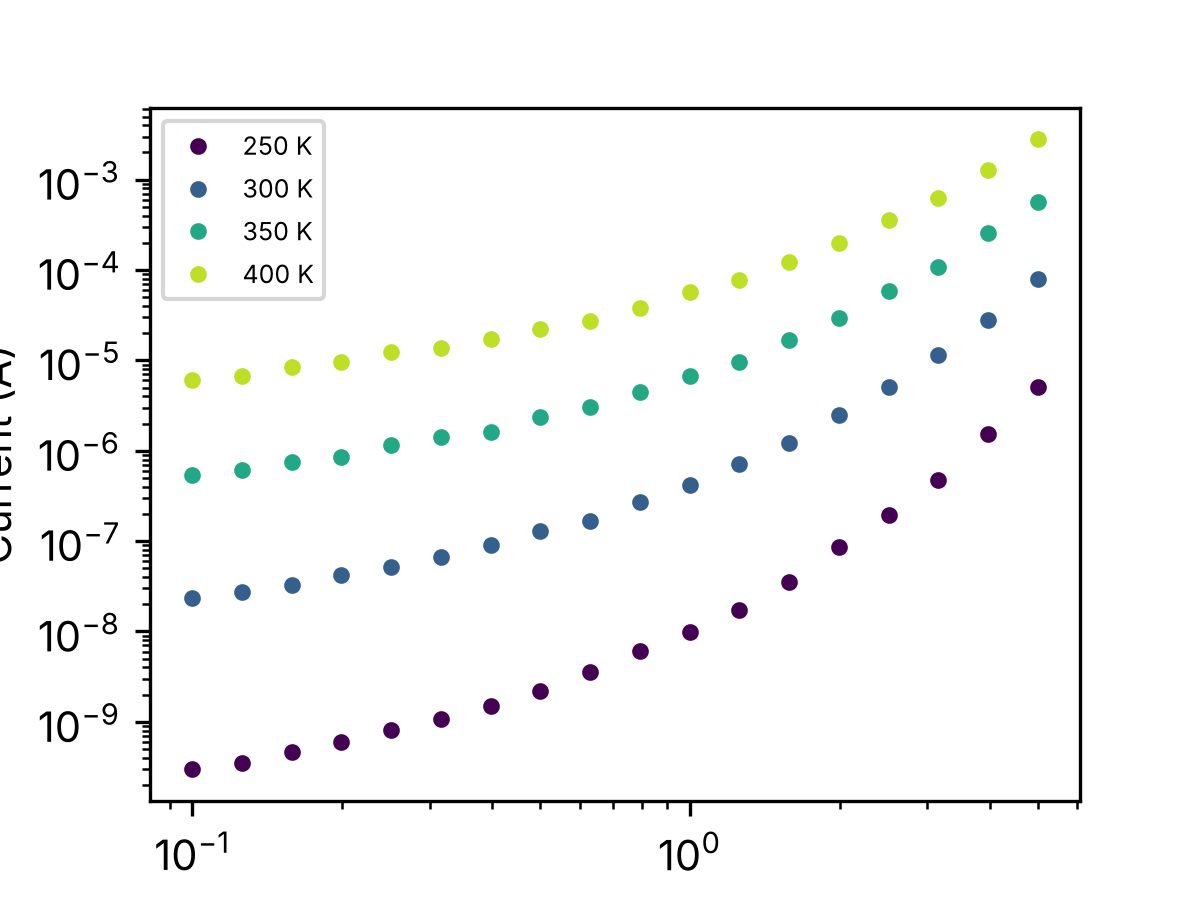
\includegraphics[width=0.78\linewidth]{mock_schottky_raster_fig.png}
\column{0.5\textwidth}
\small\textbf{Mock papers} (hidden mechanism)\\[3pt]
\scriptsize
\begin{tabular}{lll}
\toprule
Hidden & vector PDF & raster PDF\\
\midrule
Poole--Frenkel & \color{okgreen}agrees & \color{bad}disagrees$^{*}$\\
Schottky & \color{okgreen}agrees & \color{okgreen}agrees\\
Coherent & \color{okgreen}agrees & \color{cd}consistent$^{\dagger}$\\
NN hopping & \color{okgreen}agrees & \color{okgreen}agrees\\
SCLC trap & \color{okgreen}agrees & \color{cd}consistent$^{\dagger}$\\
\bottomrule
\end{tabular}\\[3pt]
\scriptsize $^{*}$overlapping markers in a low-resolution image\\
$^{\dagger}$correct mechanism among the candidates, but the digitised data cannot decide
\end{columns}
\end{frame}

% =============================================================================
\section{Benchmarks against published results}

\begin{frame}{Published systems: 8 of 8 correct}
\tiny\renewcommand{\arraystretch}{1.05}
\setlength{\tabcolsep}{4pt}\begin{tabular}{@{}lllll@{}}
\toprule
Reference & System & Mechanism & Published & BARISTA (95\,\% CI)\\
\midrule
Lenzlinger \& Snow, JAP 1969 & Al/SiO$_2$/Si & FN tunnelling & $\qE{\Phi}=3.2$ eV & $3.216\ [3.172, 3.254]$\\
Lee \emph{et al.}, APL 2011 & Au/hBN/Au & direct tunnelling & $\qE{\Phi}=3.07$ eV & $3.059\ [3.04, 3.10]$\\
Wang \emph{et al.}, PRB 2003 & Au/alkanethiol/Au & direct tunnelling & $\qE{\Phi}=1.42$ eV & $1.426\ [1.414, 1.439]$\\
Choi \emph{et al.}, JACS 2010 & ONI molecular wires & NN hopping & $\qE{E_a}=0.58$ eV & $0.580\ [0.579, 0.581]$\\
Le Corre \emph{et al.}, ACS EL 2021 & MAPbBr$_3$ crystal & SCLC, discrete trap & $\log_{10}\qN=19.1$ & $19.1$\\
Lin \emph{et al.}, PRR 2024 & graphite/CrSBr/graphite & VRH & $p=0.25$ & $0.2499\ [0.245, 0.254]$\\
Xu \emph{et al.}, PRB 1995 & a-Si:H barriers & Glazman--Matveev & $N=2$ chains & identified\\
Review, Table 8 & PF test case & Poole--Frenkel & $\qE{\Phi_t}=0.45$ eV, $\varepsilon_r=5$ & $0.4495$, $5.02$\\
\bottomrule
\end{tabular}
\vspace{8pt}

\small Every published parameter lies inside BARISTA's 95\,\% interval. Certainty grades are HIGH or VERY HIGH, except
MODERATE for Choi (single bias window).\\ Reproduce with \texttt{python benchmarks/run\_benchmarks.py}.
\end{frame}

% =============================================================================
\section{Outputs and performance}

\begin{frame}[fragile]{Manuscript-ready outputs}
\begin{columns}[T]
\column{0.5\textwidth}
\small
\textbf{Figures} (PDF, SVG, PNG at 600 dpi)
\begin{itemize}
  \item journal column widths: APS, Nature, ACS, IEEE, Elsevier, RSC
  \item embedded TrueType fonts, constrained layout, panel labels
  \item consistent colours: $\qT$ purple ramp, $\qd$ orange, $\qV$ green
  \item 15 figure types: fits, linearisations, fingerprints, model comparison, regimes, predictions, certainty, spin, trap density
\end{itemize}
\column{0.47\textwidth}
\small
\textbf{Tables and text}
\begin{itemize}
  \item \texttt{barista\_results.xlsx} + CSV for every table
  \item \texttt{parameters.tex} (booktabs) for the manuscript
  \item \texttt{methods.txt}: a ready Methods paragraph with references
  \item \texttt{report.html}: self-contained report
  \item \texttt{results.json} for scripting
\end{itemize}
\begin{lstlisting}[language=bash]
barista analyze data/ --style nature
\end{lstlisting}
\end{columns}
\end{frame}

\begin{frame}[fragile]{Fully parallel over one node --- Ibex and Shaheen}
\begin{columns}[T]
\column{0.42\textwidth}
\small
\begin{itemize}
  \item Fits, cross-validation, two-channel models, bootstrap and profiles run in a process pool
  \item Workers = cores allotted: honours \texttt{SLURM\_CPUS\_PER\_TASK}, CPU affinity, \texttt{BARISTA\_WORKERS}
  \item BLAS pinned to one thread per worker
  \item Ibex: 40 cores; Shaheen III: 192 cores
  \item Array jobs for many devices
\end{itemize}
\column{0.56\textwidth}
\begin{lstlisting}[language=bash]
#SBATCH --job-name=barista
#SBATCH --nodes=1
#SBATCH --ntasks=1
#SBATCH --cpus-per-task=40
#SBATCH --time=02:00:00

source ~/anaconda3/etc/profile.d/conda.sh
conda activate barista
export OMP_NUM_THREADS=1
export BARISTA_WORKERS=$SLURM_CPUS_PER_TASK

barista analyze "$1" --bootstrap 400 \
        -o barista_$SLURM_JOB_ID
\end{lstlisting}
\scriptsize Ready scripts in \texttt{tutorials/hpc/}: \texttt{ibex\_submit.sh}, \texttt{ibex\_array.sh},
\texttt{shaheen\_submit.sh}, \texttt{shaheen\_array.sh}.
\end{columns}
\end{frame}

\begin{frame}[fragile]{Three ways to use it}
\begin{columns}[T]
\column{0.5\textwidth}
\small\textbf{Command line}
\begin{lstlisting}[language=bash]
pip install -e ".[all]"
barista analyze iv_series.xlsx --area 100 \
        --eps-r 9 --bootstrap 200
barista spin mtj_P_AP.csv \
        --system graphene/crsb/graphene --layers 4
barista paper article.pdf
barista mechanisms      # list all models
barista gui             # Streamlit app
\end{lstlisting}
\column{0.47\textwidth}
\small\textbf{Python}
\begin{lstlisting}[language=Python]
from barista import io, engine, uncertainty
from barista.device import DeviceInfo

dev = DeviceInfo(area_um2=100, eps_r=9)
ds  = io.load("iv_series.xlsx", dev)
res = engine.analyze(ds, dev)
res.certainty = uncertainty.assess(res, B=200)
print(res.headline, res.confidence)
print(res.traps.statement)
\end{lstlisting}
\scriptsize Seven tutorials (\texttt{tutorials/01--07}): blind test, your data, two channels, single-$\qT$ traps, read a paper, graphene/CrSb/graphene spin, certainty.
\end{columns}
\end{frame}

% =============================================================================
\begin{frame}{Limitations and next steps}
\begin{columns}[T]
\column{0.5\textwidth}
\begin{alertblock}{Limitations}
\small
\begin{itemize}
  \item Bias-only data cannot identify a mechanism uniquely; BARISTA says so.
  \item SCLC trap densities scale with $\varepsilon_r$; TAT densities with $\nu_0$ --- supply them when known.
  \item Raster figures with overlapping markers can mislead the digitiser.
  \item Spin models assume collinear magnetisation (P/AP or angle).
\end{itemize}
\end{alertblock}
\column{0.47\textwidth}
\begin{exampleblock}{Next}
\small
\begin{itemize}
  \item Benchmark on more user-supplied papers with raw data
  \item Noise (RTN) and impedance inputs for trap spectroscopy
  \item Gate-dependent data (field-effect barriers)
  \item Bayesian evidence via nested sampling as an option
\end{itemize}
\end{exampleblock}
\end{columns}
\end{frame}

\begin{frame}{Summary}
\begin{itemize}
  \item \textbf{One input, one verdict}: any file or paper $\to$ mechanism, parameters and how certain both are.
  \item \textbf{Physics first}: 13 mechanisms with global $\qI(\qV,\qT,\qd)$ fits, model-free fingerprints, plausibility checks.
  \item \textbf{Statistics that answer ``how sure?''}: bootstrap selection probability, profile likelihood, Vuong tests.
  \item \textbf{Trap density from I--V}: $\qN$ and its energy for every trap-related mechanism, or a bound when no traps are needed.
  \item \textbf{Spin}: spin filtering, spin hopping, interface proximity polarisation (graphene/CrSb/graphene), Valet--Fert.
  \item \textbf{Validated}: 8/8 published systems, 4/4 spin benchmarks, digitiser errors $\leq$\,2\,\%.
  \item \textbf{Ready to publish and to scale}: journal-style figures, \LaTeX\ tables, one-node parallel on Ibex/Shaheen.
\end{itemize}
\vfill
\centering
\href{https://github.com/Gokaran-Shukla/barista}{\texttt{github.com/Gokaran-Shukla/barista}} \quad MIT licence
\end{frame}

\end{document}
